% =========================================================================== %

\begin{frame}[t,plain]
\titlepage
\end{frame}

% =========================================================================== %

\begin{frame}{Recap}
%
\begin{columns}[t]
\column{.5\linewidth}
\begin{itemize}
\item Subplots in matplotlib
	\begin{itemize}
	\item \texttt{plt.subplot} and \texttt{fig.add\_subplot}
	\item Option: Polar plot
	\end{itemize}
\item Object oriented approach
	\begin{itemize}
	\item Figures (Windows)
	\item Axes Objects (Subplots)
	\item Tons of Methods
	\item Getters and Setters
	\end{itemize}
\item Gridspecs
	\begin{itemize}
	\item Invisible Grid
	\item Subsections selectable via slicing syntax
	\end{itemize}
\end{itemize}
%
\column{.5\linewidth}
\begin{itemize}
\item Tickmarks
	\begin{itemize}
	\item List of poositions
	\item List of strings or dynamic generation
	\end{itemize}
\item \LaTeX~ in MatPlotLib
\item Text Overlays and Arrows
\item 3D Plots
	\begin{itemize}
	\item True 3D plots with \texttt{mpl\_toolkits.mplot3d.Axes3D}
	\item Pseudo-3D plots with colourmaps
	\end{itemize}
\item Saving plots
\end{itemize}

\end{columns}
%
\begin{center}
	\emph{Any Questions?}
\end{center}
%
\end{frame}

% =========================================================================== %

\begin{frame}[fragile]{Chapter 11}
%
\begin{itemize}
\item NumPy Arrays
\item Index Access
\item Quick Generation of Numpy Arrays
\item Meshgrids
\item Broadcasting Operators and Functions
\item Transpositions
\end{itemize}
%
\end{frame}

% =========================================================================== %

\begin{frame}[fragile]{Recap: Memory Structure in Python}
%
\begin{itemize}
\item Everything belongs to class \texttt{Object}
	\begin{itemize}
	\item Descriptor: Collection of metadata on how to interpret the object
	\item Reference to class in particular
	\item Reference to useful data
	\item[\Thus] At least two jumps in memory per access to any piece of information
	\end{itemize}
\item Everything is handled via references
	\begin{itemize}
	\item \inPy{list}: List of reference to descriptors
	\item High flexibility
	\end{itemize}
\item Runtime aspect
	\begin{itemize}
	\item Some operations very quick (\eg sorting)
	\item But, generally: flexibility at cost of speed
	\end{itemize}
\item[\Thus] What if we cut into flexibility?
\item[\Thus] NumPy does exactly that
\end{itemize}
%
\end{frame}

% =========================================================================== %

\begin{frame}[fragile]{NumPy -- Convention and Installation}
%
\begin{itemize}
\item Numpy should be installed on your machines
\item If so: Convention \inPy{import numpy as np} 
	\begin{itemize}
	\item In this lecture: often omitted
	\end{itemize}
\end{itemize}
%
\begin{codebox}[Test for Installation]
\begin{minted}[linenos, fontsize=\scriptsize]{python3}
try                : import numpy as np
except ImportError : print("numpy is not installed")
else               : print("numpy is ready for use")
\end{minted}
\end{codebox}
%
\begin{cmdbox}[Install]
\begin{minted}[fontsize=\scriptsize]{text}
conda install numpy  # Anaconda users
pip install numpy    # Windows users with other environment manager
pip3 install numpy   # Linux users
\end{minted}
\end{cmdbox}
%
\end{frame}

% =========================================================================== %

\begin{frame}[fragile]{The Primary Object}
%
\begin{itemize}
\item \texttt{np.ndarray}: Collection of objects of \emph{same type}
\item Preferred: \emph{primitve types} (types that are so simple that the processor itself \enquote{understands} them)
	\begin{itemize}
	\item Integers, floating point numbers and complex numbers, but ...
	\item ... fixed width
	\item \texttt{np.intX}, \texttt{np.floatX} and \texttt{np.complexX} where \texttt{X} is number of bits
	\item Usually: \texttt{np.int64}, \texttt{np.float64}, \texttt{np.complex128}
	\end{itemize}
\item Function \texttt{np.array} converts Python iterables into \texttt{np.ndarray}
	\begin{itemize}
	\item Works also with lists of lists of lists of lists ...
	\item ... if full dimension is given
	\item Otherwise: Fallback solutions with less efficient handling
	\end{itemize}
\item Implicit type conversion
	\begin{itemize}
	\item Integer \thus floating point number \thus string \thus object
	\end{itemize}
\end{itemize}
%
\end{frame}

% =========================================================================== %

\begin{frame}[fragile]
%
\vspace{-2pt}
\begin{tcbraster}[raster columns=2,
                  raster equal height,
                  nobeforeafter,
                  raster column skip=0.5cm]
\begin{codebox}[Example: Creating NumPy Arrays]
\begin{minted}[linenos, fontsize=\scriptsize]{python3}
import numpy as np

npList = np.array([1, 2, 3])
npMixed1 = np.array([1, 1.5])
npMixed2 = np.array([1, 1.0, "1.0"])

npTab = np.array([[1, 2, 3], [4, 5, 6]])
npListList = np.array([[1], [2, 3]])

print(npList)
print(npMixed1)
print(npMixed2)
print(npTab)
print(npListList)
\end{minted}
\end{codebox}
%
\begin{cmdbox}[Output: Creating NumPy Arrays]
\begin{minted}[fontsize=\scriptsize]{text}
[1 2 3]
[1. 1.5]
['1' '1.0' '1.0']
[[1 2 3]
 [4 5 6]]
[list([1]) list([2, 3])]
\end{minted}
\end{cmdbox}
\end{tcbraster}
%
\begin{hintbox}[Display of Matrices and Tensors]
\footnotesize
Note how the output of \texttt{npTab} is in two lines and already looks like a matrix!\\
This also works with tensors of any rank (though it doesn't look nearly as nice...)
\end{hintbox}
%
\end{frame}

% =========================================================================== %

\begin{frame}[fragile]{Simple Attributes of \texttt{np.ndarray}}
%
\begin{itemize}
\item \texttt{dtype} -- underlying data type (\eg \texttt{np.int64})
	\begin{itemize}
	\item Can be used to force type
	\item \inPy{data = np.array([1, 2, 3], dtype=np.float64)}
	\end{itemize}
\item \texttt{shape} -- \inPy{tuple} of elements per dimension
	\begin{itemize}
	\item E.\;g. simple list: \inPy{tuple} with one element: lenght of list
	\item E.\;g. matrix: \inPy{tuple} with two elements: width and height
	\end{itemize}
\item \texttt{size}: total of elements in the \texttt{np.ndarray}
	\begin{itemize}
	\item \texttt{array.size == prod(array.shape)}
	\end{itemize}
\item \texttt{ndim}: number of dimensions in the \texttt{np.ndarray}
	\begin{itemize}
	\item \texttt{array.ndim == len(array.shape)}
	\end{itemize}
\item \texttt{data}: where in memory to find the actual data
	\begin{itemize}
	\item Can be used with \inPy{memoryview} class
	\item Mostly for advanced techniques and communication with external libraries
	\end{itemize}
\end{itemize}
%
\end{frame}

% =========================================================================== %\\

\begin{frame}[fragile]{Index Access to \texttt{np.ndarray}}
%
\begin{itemize}
\item Same options as regular \inPy{list}s
	\begin{itemize}
	\item \inPy{int}s from 0 to N-1
	\item Negative indices from -1 to -N
	\item Slices (\texttt{start : stop : stride} with optional arguments (\texttt{start :: stride})
	\end{itemize}
\item (Implicit) \inPy{tuple}s instead of multiple brackets
	\begin{itemize}
	\item \texttt{array[a, b]} is equivalent to \texttt{array[a][b]}
	\item \texttt{array[:, b]} is \emph{all rows, column \texttt{b}}
	\item \texttt{array[a:b, c:d]} is sub-matrix rows \texttt{a} to \texttt{b}, columns \texttt{c} to \texttt{d}
	\end{itemize}
\item \inPy{list}s or \texttt{np.ndarray}s of \inPy{int}s: multiple selections in one go
	\begin{itemize}
	\item Creates an \texttt{np.ndarray} with one dimension more than the selected objects
	\item[\Thus] Collection of selections
	\end{itemize}
\item \inPy{list}s or \texttt{np.ndarray}s of \inPy{bool}s: bitmask (irregular selection)
	\begin{itemize}
	\item One \inPy{True} for each selected
	\item Needs to be of same length as list
	\item May be used with multidimensional \texttt{np.ndarray}s; flattens tensors
	\end{itemize}
\end{itemize}
%
\end{frame}

% =========================================================================== %

\begin{frame}[fragile]
%
\begin{tcbraster}[raster columns=2,
                  raster equal height,
                  nobeforeafter,
                  raster column skip=0.2cm]
\begin{codebox}[Example: Index Access ...]
\begin{minted}[linenos, fontsize=\scriptsize]{python3}
npTab = np.array([[ 1,  2,  3],
                  [ 4,  5,  6],
                  [ 7,  8,  9],
                  [10, 11, 12]])

print("entire table:\n", npTab)
print()

print("element (0, 1):", npTab[0, 1])
print()

print("last row:"      , npTab[-1])
print("column 1:"      , npTab[:,1])
print()

print("upper left square:\n",
      npTab[0:2, 0:2])
\end{minted}
\end{codebox}
%
\begin{cmdbox}[Output: Index Access]
\begin{minted}[fontsize=\scriptsize]{text}
entire table:
[[ 1  2  3]
 [ 4  5  6]
 [ 7  8  9]
 [10 11 12]]
 
element (0, 1): 2

last row: [10 11 12]
column 1: [ 2  5  8 11]

upper left square:
 [[1 2]
 [4 5]]
\end{minted}
\end{cmdbox}
\end{tcbraster}
%
\end{frame}

% =========================================================================== %

\begin{frame}[fragile]
%
\begin{tcbraster}[raster columns=2,
                  raster equal height,
                  nobeforeafter,
                  raster column skip=0.2cm]
\begin{codebox}[... continued]
\begin{minted}[linenos, firstnumber=18, fontsize=\scriptsize]{python3}
print("second and last row:\n",
      npTab[[1,-1]])
print()

print("two matrices:\n",
      npTab[
            np.array([[1, 2], [2, 1]])
           ])
print()

mask = [True, False, True, False]
print("1D mask:\n",
      npTab[mask])
print()

mask = np.array([[ True, False,  True],
                 [False,  True, False],
                 [ True, False,  True],
                 [False,  True, False]])
print("2D mask:\n", npTab[mask])
\end{minted}
\end{codebox}
%
\begin{cmdbox}[... continued]
\begin{minted}[fontsize=\scriptsize]{text}
second and last row:
[[ 4  5  6]
 [10 11 12]]

two matrices:
[[[4 5 6]
  [7 8 9]]

 [[7 8 9]
  [4 5 6]]]

1D mask:
[[1 2 3]
 [7 8 9]]

2D mask:
 [ 1  3  5  7  9 11]
\end{minted}
\end{cmdbox}
\end{tcbraster}
%
\end{frame}

% =========================================================================== %

\begin{frame}[fragile]{Quickly Creating \texttt{np.ndarray}s}
%
\begin{itemize}
\item \texttt{np.arange(start, stop, stride)} -- like \inPy{range}, but works with \inPy{float}s as well
	\begin{itemize}
	\item Same meaning of parameters
	\item one-parameter form means \enquote{from 0 to parameter in steps of one}
	\end{itemize}
\item \texttt{np.linspace(start, stop, N = 50)} -- similar, but with number of elements
	\begin{itemize}
	\item Last element \emph{included}
	\item \inPy{np.linspace(5, 20, 4) == np.array([5, 10, 15, 20])}
	\end{itemize}
\item \texttt{np.geomspace(start, stop, N = 50)}
	\begin{itemize}
	\item Like \texttt{linspace}, but constant (\emph{factor} instead of \emph{difference})
	\end{itemize}
\item \texttt{np.logspace(exp1, exp2, N = 50, base=10)}
	\begin{itemize}
	\item Like \texttt{geomspace}, but with explicit \texttt{base} and \texttt{exp}onents
	\item Generates $base^{exp1} ~...~ base^{exp2}$
	\end{itemize}
\item For all:
	\begin{itemize}
	\item Optional parameter \texttt{dtype} allows to force data type
	\end{itemize}
\end{itemize}
%
\end{frame}

% =========================================================================== %

\begin{frame}[fragile]{Quickly Creating Even More \texttt{np.ndarray}s}
%
\begin{itemize}
\item \texttt{np.zeros(size)} -- creates an \texttt{np.ndarray} filled with zeros
\item \texttt{np.ones(size)} -- guess what
\item \texttt{np.fill(size, value)} --  creates an \texttt{np.ndarray} filled with one given \texttt{value}
\item For all:
	\begin{itemize}
	\item \texttt{size} may be an \inPy{int}eger (creates a list of length \texttt{size}) ...
	\item ... or a \inPy{tuple} (creates a tensor of dimensions \texttt{size})
	\item Optional argument \texttt{dtype} as usual
	\end{itemize}
\end{itemize}
%
\end{frame}

% =========================================================================== %

\begin{frame}[fragile]{For Good Measure: Quickly Creating Still More \texttt{np.ndarray}s}
%
\begin{itemize}
\item \texttt{np.identity(size)} -- creates identity matrix
	\begin{itemize}
	\item \texttt{size} must be an \texttt{integer}
	\item Matrix with all zeros, except for principal diagonal where there are ones
	\item Optional argument \texttt{dtype} as usual
	\end{itemize}
\item \texttt{np.eye(N, M, k=0)} -- creates non-square matrix like identity
	\begin{itemize}
	\item Size of matrix will be $N \times M$
	\item Ones will be on $k^{\text{th}}$ diagonal
	\item Optional argument \texttt{dtype} as usual
	\end{itemize}
\item \texttt{np.diag(obj, k)}
	\begin{itemize}
	\item If \texttt{obj} is a 1D array: create a diagonal matrix with \texttt{obj} on the $k\texttt{\text{th}}$ diagonal
	\item If \texttt{obj} is a 2D array: extract the $k\texttt{\text{th}}$ diagonal as a 1D array
	\item \emph{No} optional argument \texttt{dtype}!
	\end{itemize}
\end{itemize}
%
\end{frame}

% =========================================================================== %

\begin{frame}[fragile]
%
\begin{tcbraster}[raster columns=2,
                  raster equal height,
                  nobeforeafter,
                  raster column skip=0.2cm]
\begin{codebox}[Example: Quick \texttt{np.ndarray}s]
\begin{minted}[linenos, fontsize=\scriptsize]{python3}
print(np.arange(5))
print(np.arange(0, 2, 0.25))
print(np.arange(5, 10, dtype=np.float64),
      end="\n\n" )
print(np.linspace(0, 1.8, 10))
print(np.geomspace(2, 256, 8))
print()
print(np.zeros(5) )
print(np.fill((2, 2), 3.14))

print()
print(np.identity(1))
print(np.identity(3,dtype=np.int64))


print( np.eye(2, 4) )

\end{minted}
\end{codebox}
%
\begin{cmdbox}[Output: Quick \texttt{np.ndarray}s]
\begin{minted}[fontsize=\scriptsize]{text}
[0 1 2 3 4]
[0.   0.25 0.5  0.75 1.   1.25 1.5  1.75]
[5. 6. 7. 8. 9.]

[0.  0.2 0.4 0.6 0.8 1. 1.2 1.4 1.6 1.8]
[  2.   4.   8.  16.  32.  64. 128. 256.]

[0. 0. 0. 0. 0.]
[[3.14 3.14]
 [3.14 3.14]]

[[1.]]
[[1 0 0]
 [0 1 0]
 [0 0 1]]
[[1. 0. 0. 0.]
 [0. 1. 0. 0.]]
\end{minted}
\end{cmdbox}
\end{tcbraster}
%
\end{frame}

% =========================================================================== %

\begin{frame}[fragile]
%
\begin{tcbraster}[raster columns=2,
                  raster equal height,
                  nobeforeafter,
                  raster column skip=0.2cm]
\begin{codebox}[Example: Quick \texttt{np.ndarray}s]
\begin{minted}[linenos, fontsize=\scriptsize]{python3}
npList = np.array([1, 2, 3])
npTab  = np.array([[ 1,  2,  3],
                   [ 4,  5,  6],
                   [ 7,  8,  9],
                   [10, 11, 12]])

print(diag(npList), end='\n' * 5)
print(np.diag(npTab))
print(np.diag(npTab, 1))
print(np.diag(npTab, -1) )
\end{minted}
\end{codebox}
%
\begin{cmdbox}[Output: Quick \texttt{np.ndarray}s]
\begin{minted}[fontsize=\scriptsize]{text}
[[1 0 0]
 [0 2 0]
 [0 0 3]]




[1 5 9]
[2 6]
[ 4 8 12]
\end{minted}
\end{cmdbox}
\end{tcbraster}
%
\end{frame}

% =========================================================================== %

\begin{frame}{Meshgrids}
%
\begin{itemize}
\item Imagine several collections of values
	\begin{itemize}
	\item E.\;g. \texttt{[red, green, blue]} and \texttt{[+1, -1]}
	\item Or more than two containers
	\end{itemize}
\item Want: all combinations of these items
	\begin{itemize}
	\item E.\;g. \texttt{[(red, +1), (red, -1), (green, +1), (green, -1), (blue, +1), (blue, -1)]}\\
	\item Or more than two items per tuple
	\end{itemize}
\item That's what \texttt{np.meshgrid}s are good for
\item But (for good reasons): Return as separate lists
	\begin{itemize}
	\item \texttt{[red, red, green, green, blue, blue]} and \texttt{[+1, -1, +1, -1, +1, -1]}
	\item Can still be \inPy{zip}ped to \inPy{tuple}s
	\end{itemize}
\end{itemize}
%
\end{frame}

% =========================================================================== %

\begin{frame}[fragile]{Meshgrids and Index Meshgrids -- Syntax}
%
\begin{codebox}[Syntax: Creating Meshgrids]
\begin{minted}[fontsize=\scriptsize]{python3}
allCombos = np.meshgrid(pool1, pool2, ...)
\end{minted}
\end{codebox}
%
\begin{itemize}
\item \texttt{pool1}, \texttt{pool2}, ... are the collections from before (\eg \texttt{[red, green, blue]})
\item \texttt{allCombos} is a \inPy{list} of \texttt{np.ndarray}s
\item Often used with tuple unpacking:\\
	\inPy{X, Y = np.meshgrid( np.linspace(0.2, 10), np.linspace(0.4, 20) )}
\item Special form: Index meshgrids: \inPy{int}s from 0 to some upper boundaries
\item Command \texttt{np.indices(dimensions)}
\item \texttt{dimensions} is a \inPy{tuple} with the number of elements per dimension
\item E.\;g.: \inPy{I, J = np.indices( (50, 50) )}
\end{itemize}
%
\end{frame}

% =========================================================================== %

\begin{frame}[fragile]{Broadcasting -- Computing with \texttt{np.ndarray}s}
%
\begin{itemize}
\item Between two \texttt{np.ndarray}s (\texttt{v <op> u})
	\begin{itemize}
	\item Element-Wise operations for all primary operators (+, -, *, /, **, \%)
	\item \texttt{np.array([1, 2, 3]) + np.array([3, 2, 1]) == np.array([4, 4, 4])}
	\item Matrix multiplication with \texttt{@} (if fitting dimensions)
	\item Dot product for 1D arrays (\texttt{np.outer} gives the tensor product)
	\item Also works with tensors
	\end{itemize}
\item Between \texttt{np.ndarray} and some scalar, \eg an \inPy{int} (\texttt{u <op> s} or \texttt{s <op> u})
	\begin{itemize}
	\item Operation for each element
	\item \texttt{np.array([1, 2, 3]) + 1 == np.array([2, 3, 4])}
	\item Same operators plus assignment
	\item Can be used with slices and bitmasks
	\end{itemize}
\end{itemize}
%
\end{frame}

% =========================================================================== %

\begin{frame}[fragile]{Broadcasting -- Functions on \texttt{np.ndarray}s}
%
\begin{itemize}
\item \texttt{np.ndarray}s are \emph{iterable}
	\begin{itemize}
	\item \inPy{for x in np.linspace(0.2, 10) : ...} works
	\end{itemize}
\item Computing $f(x)$ for each $x$ in a \texttt{np.ndarray} is possible with that ...
\item ... but doesn't exploit the regular structure of \texttt{np.ndarray}s
\item Instead: common functions from module \texttt{math} re-written in \texttt{numpy}
\item \texttt{np.sin(array)} computes $\sin(x)$ for each $x$ in \texttt{array}
\item Much faster than \texttt{for}-loop (albeit internally a \texttt{for}-loop, too)
\end{itemize}
%
\end{frame}

% =========================================================================== %

\begin{frame}[fragile]
%
\vspace{-8pt}
\begin{tcolorbox}[title=Differential Quotient]
	\begin{equation*}
	\dv{x} f(x)
=
	\lim_{\varepsilon \to 0}
		\frac
			{f(x + \varepsilon) - f(x)}
			{\varepsilon}
	\end{equation*}
\end{tcolorbox}
%
\vspace{-3pt}
\begin{codebox}[Example: Numerical Derivative, width=.6\linewidth, nobeforeafter, equal height group = grpXmpNumPyDerivative]
\begin{minted}[linenos, fontsize=\scriptsize]{python}
import numpy as np
import matplotlib.pyplot as plt

X1 = np.linspace(0, 2 * np.pi)
Y1 = np.sin(X1)
X2 = (X1[1:] + X1[:-1]) / 2
Y2 = (Y1[1:] - Y1[:-1]) / (X1[1:] - X1[:-1])

plt.figure()
plt.plot(X1, Y1, label="sine")
plt.plot(X2, Y2, label="derivative of sine")
plt.legend()
plt.plot()
\end{minted}
\end{codebox}
%
\begin{tcolorbox}[title=Example: Num. Derivative, width=.39\linewidth, nobeforeafter, equal height group = grpXmpNumPyDerivative]
\hspace{-14pt}
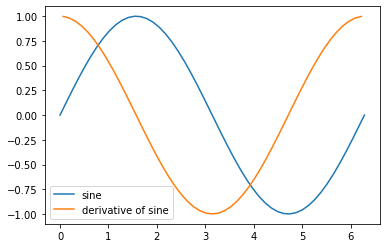
\includegraphics[width=1.2\linewidth]{./gfx/np-derivative}
\end{tcolorbox}
%
\end{frame}

% =========================================================================== %

\begin{frame}[fragile]
%
\begin{hintbox}[np.gradient]
The function \texttt{np.gradient} is both, more flexible and more robust against numerical fluctuations than the method shown above. It can compute the gradient of scalar fields as well or do multiple derivatives in parallel. (However, the basic principle is the same.)

\vspace{3pt}
The example above is primarily meant to show how array operations are performed with NumPy.
\end{hintbox}
%
\end{frame}

% =========================================================================== %

\begin{frame}[fragile]
%
\begin{tcbraster}[raster columns=2,
                  raster equal height,
                  nobeforeafter,
                  raster column skip=0.5cm]
\begin{codebox}[Example: Batch Computation]
\begin{minted}[linenos, fontsize=\scriptsize]{python3}
import numpy as np
import matplotlib.pyplot as plt
from mpl_toolkits.mplot3d import Axes3D

xVals = np.linspace(-2*np.pi, 2*np.pi,
                    201)
yVals = np.linspace(-2*np.pi, 2*np.pi,
                    201)

X, Y = np.meshgrid(xVals, yVals)

Z = 0.2 * np.sqrt(X**2 + Y**2) * \
          np.cos(X) * np.sin(Y)

fig = plt.figure()
drw = fig.add_subplot(projection='3d')
drw.plot_surface(X, Y, Z)
drw.view_init(60, 45)
plt.show()
\end{minted}
\end{codebox}
%
\begin{tcolorbox}[title=Output: Batch Computation]
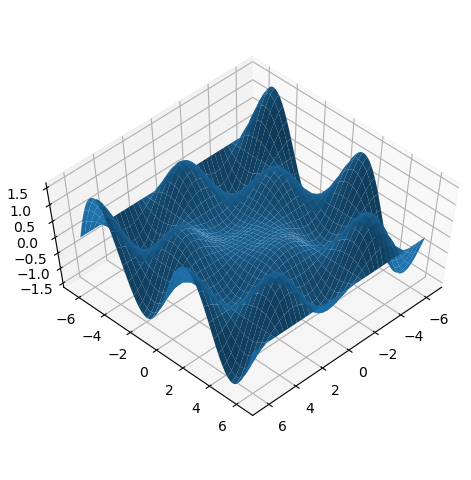
\includegraphics[width=\linewidth]{./gfx/np-wave}
\end{tcolorbox}
\end{tcbraster}
%
\end{frame}

% =========================================================================== %

\begin{frame}[fragile]{Comparisons}
%
\begin{itemize}
\item Comparison operators (\texttt{==}, \texttt{!=}, \texttt{<}, \texttt{<=}, ...) are evaluated element-wise, too
	\begin{itemize}
	\item Works both, between two \texttt{np.ndarray}s or between a \texttt{np.ndarray} and a scalar.
	\end{itemize}
\item Return type: \texttt{np.ndarray} of \inPy{bool}s \Thus Bitmask
	\begin{itemize}
	\item Remember: bitmasks can be used for write access, too
	\end{itemize}
\item Check for equality of entire array
	\begin{itemize}
	\item Manually: \inPy{u.shape == v.shape and all(u == v)}
	\item \inPy{all}: logical \inPy{and} of all array elements
	\item related: \inPy{any}: logical \inPy{or} of all array elements
	\item Better: \texttt{np.all} and \texttt{np.any} -- exploits regular structure, works faster
	\item Still better and simpler: \texttt{np.array\_equal(u, v)} (does the same steps)
	\end{itemize}
\end{itemize}
%
\end{frame}

% =========================================================================== %

\begin{frame}[fragile]
%
\vspace{-1pt}
\begin{tcbraster}[raster columns=2,
                  raster equal height,
                  nobeforeafter,
                  raster column skip=0.2cm]
\begin{codebox}[Example: Compare Operation]
\begin{minted}[linenos, fontsize=\scriptsize]{python3}
import numpy as np
import matplotlib.pyplot as plt

X = np.linspace(0, 2 * np.pi)
Y = np.sin(X)

mask = np.abs(Y) > 0.5

Y[mask] = 1 - Y[mask]
Y[Y > 1] = -0.5

plt.figure()
plt.plot(X, Y)
plt.show()
\end{minted}
\end{codebox}
%
\begin{tcolorbox}[title=Output: Compare Operation]
\hspace{-14pt}
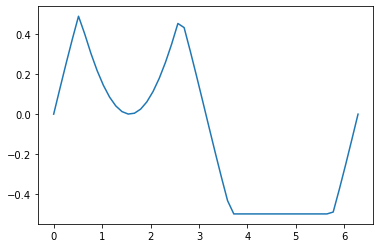
\includegraphics[width=1.15\linewidth]{./gfx/np-comp}
\end{tcolorbox}
\end{tcbraster}
%
\vspace{-9pt}
\begin{hintbox}[Usage of Batch Comparisons]
\footnotesize
Use this to filter for special values, \eg invalid values, surpassing a threshold value, steepest region, ...
\end{hintbox}
%
\end{frame}

% =========================================================================== %

\begin{frame}[fragile]{Transpositions}
%
\begin{itemize}
\item Transposition of a matrix
	\begin{itemize}
	\item \enquote{Flipping it around the principal diagonal}
	\item Swapping the role of the row- and column index
	\end{itemize}
\item Generalization for tensors
	\begin{itemize}
	\item Any permutation of the order of indices
	\item E.\;g. $A_{i, j, k} \to A_{k, i, j}$
	\end{itemize}
\item In NumPy
	\begin{itemize}
	\item Attribute \texttt{T}: inversion of indices ($i, j, k \to k, j, i$)
	\item \texttt{A.T.T == A}
	\item Method \texttt{transpose} for generic permutation of indices
	\item \texttt{A.transpose(index\_0, index\_1, ...)}
	\item E.\;g. $A_{i, j, k} \to A_{k, i, j}$: \texttt{A.transpose(2, 0, 1)}
	\end{itemize}
\end{itemize}
%
\end{frame}

% =========================================================================== %
